\documentclass[12pt, a4paper]{article}

\usepackage{fullpage}
\usepackage{latexsym}
\usepackage{amsfonts}
\usepackage{amssymb}
\usepackage{graphicx}
\usepackage{amsmath}
\usepackage{float}
\usepackage{subcaption}

\pagestyle{empty}

\begin{document}

\title{{AMATH 568\\
Advanced Differential Equations}\\
{\bf \Huge Homework 6}}

\author{Lucas Cassin Cruz Burke}

\date{Due: February 24, 2023}

\maketitle

\begin{enumerate}
    \item Consider the singular equation: $$\epsilon y'' + (1+x)^2 y' + y = 0$$
    
    with $y(0)=y(1)=1$ and with $0<\epsilon \ll 1$. 

    \begin{enumerate}
        \item Obtain the leading order uniform solution using the WKB method. 
        
        \textbf{Solution:} We begin by making the WKB ansatz $$y(x) = e^{S(x)/\delta},$$ where $S(x) = S_0(x) + \delta S_1(x) + \dots$ and $0 < \delta \ll 1$. We can calculate the relevant derivatives to $\mathcal O (1)$ as 

        \begin{align*}
            y' &= \frac{S'}{\delta} y = \left(\frac{1}{\delta}S_0' + S_1'\right) y \\ y'' &= \left( \frac{S''}{\delta}  + \frac{{S'}^2}{\delta^2} \right) y = \left( \frac{1}{\delta}(S_0'' + \delta S_1'') + \frac{1}{\delta^2}({S_0'}^2 + 2\delta S_0'S_1') \right) y \\
            &= \left( \frac{1}{\delta^2} {S_0'}^2 + \frac{1}{\delta}(S_0'' + 2 S_0'S_1') + S_1'' \right) y
        \end{align*}

        Plugging our ansatz into the above singular equation results in the following condition for $y(x) \ne 0$:

        \begin{align*}
            \epsilon \left( \frac{S''}{\delta}  + \frac{{S'}^2}{\delta^2} \right) + (1+x)^2 \frac{S'}{\delta} + 1 &=0 \\
            \Rightarrow \epsilon \left( \frac{1}{\delta^2} {S_0'}^2 + \frac{1}{\delta}(S_0'' + 2 S_0'S_1') + S_1'' \right) + (1+x)^2 \left(\frac{1}{\delta}S_0' + S_1'\right) + 1 &=0
        \end{align*}

        To leading order, we have the terms $$\frac{\epsilon}{\delta^2} {S_0'}^2 + (1+x)^2 \frac{1}{\delta} S_0' = 0$$

        Hence, to establish a dominant balance we require that

        $$\frac{\epsilon}{\delta^2} \sim \frac{1}{\delta},$$

        which we can satisfy by setting $\delta = \epsilon$. 

        With this, our equation for $S(x)$ becomes, to leading order $\mathcal O(1/\epsilon)$, 

        \begin{align*}
            {S_0'}^2 + (1+x)^2 S_0' = 0 
        \end{align*}

        This is trivially satisfied when $S_0'=0 \Rightarrow S_0 = C$. In this case, our governing equation becomes, to $\mathcal O(1)$, 

        \begin{align*}
            (1+x)^2 S_1' + 1 = 0 \\ S_1' = \frac{-1}{(1+x)^2} \\ \Rightarrow S_1 = \frac{1}{1+x}
        \end{align*}

        and we find the WKB solution 

        $$y(x) = C_1 \exp \left[  \frac{1}{1+x} \right]$$
        
        If $S_0' \ne 0$, we have 

        \begin{align*}
            S_0' = -(1+x)^2 \Rightarrow S_0 = - \frac{1}{3} (1+x)^3 + C
        \end{align*}

        In this case we have, to $\mathcal O(1)$, 

        \begin{align*}
            S_0'' + 2 S_0' S_1' + (1+x)^2 S_1' &= 0 \\
            \Rightarrow -2(1+x) -2(1+x)^2 S_1' + (1+x)^2 S_1' &= 0 \\
            \Rightarrow -2(1+x) - (1+x)^2 S_1' &= 0 \\
            \Rightarrow S_1' = \frac{-2}{1+x} \Rightarrow S_1 = \log \left[ \frac{1}{(1+x)^2} \right]
        \end{align*}

        Hence we find the WKB solution 

        $$y(x) = \frac{C_2}{(1+x)^2} \exp \left[ - \frac{1}{3\epsilon} (1+x)^3  \right]$$

        We can now combine these two solutions to find

        \begin{align*}
            y(x) = C_1 \exp \left[  \frac{1}{1+x} \right] + \frac{C_2}{(1+x)^2} \exp \left[ - \frac{1}{3\epsilon} (1+x)^3  \right]
        \end{align*}

        Our boundary conditions require that $y(0) = 1$, which gives us 

        \begin{align*}
            y(0)= C_1 e + C_2 e^{-1/3\epsilon} = 1 && \Rightarrow && C_2 = e^{1/3\epsilon}(1-C_1 e)
        \end{align*}

        And our second boundary condition requires that $y(1) =1$, which gives us 

        \begin{align*}
            y(1) = C_1 e^{1/2} + \frac{C_2}{4} e^{-8/3\epsilon} &= 1 \\
            C_1 e^{1/2} + \frac{1}{4} (1-C_1 e) e^{-7/3\epsilon} &= 1 \\
            C_1 \left( e^{1/2} - \frac{1}{4} e^{1-\frac{7}{3\epsilon}}\right) &= 1 - \frac{1}{4} e^{-7/3\epsilon} \\
            C_1 &= \left( 1 - \frac{1}{4} e^{-7/3\epsilon} \right) \left( e^{1/2} - \frac{1}{4} e^{1-\frac{7}{3\epsilon}}\right)^{-1}
        \end{align*}

        All together, our final WKB uniform solution is given to leading order by 

        \begin{align*}
            y(x) =  A(\epsilon) \exp \left[  \frac{1}{1+x} \right] +  \frac{e^{\frac{1}{3\epsilon}} (1-e A(\epsilon))}{(1+x)^2} \exp \left[ - \frac{1}{3\epsilon} (1+x)^3  \right],
        \end{align*}

        where $$A(\epsilon) = \left( 1 - \frac{1}{4} e^{-7/3\epsilon} \right) \left( e^{1/2} - \frac{1}{4} e^{1-\frac{7}{3\epsilon}}\right)^{-1}$$

        \clearpage 
        \item Plot the uniform solution for $\epsilon = 0.01,0.05,0.1,0.2$. 
        
        \textbf{Solution:} 
        
        \begin{figure}[H]
            \centering
            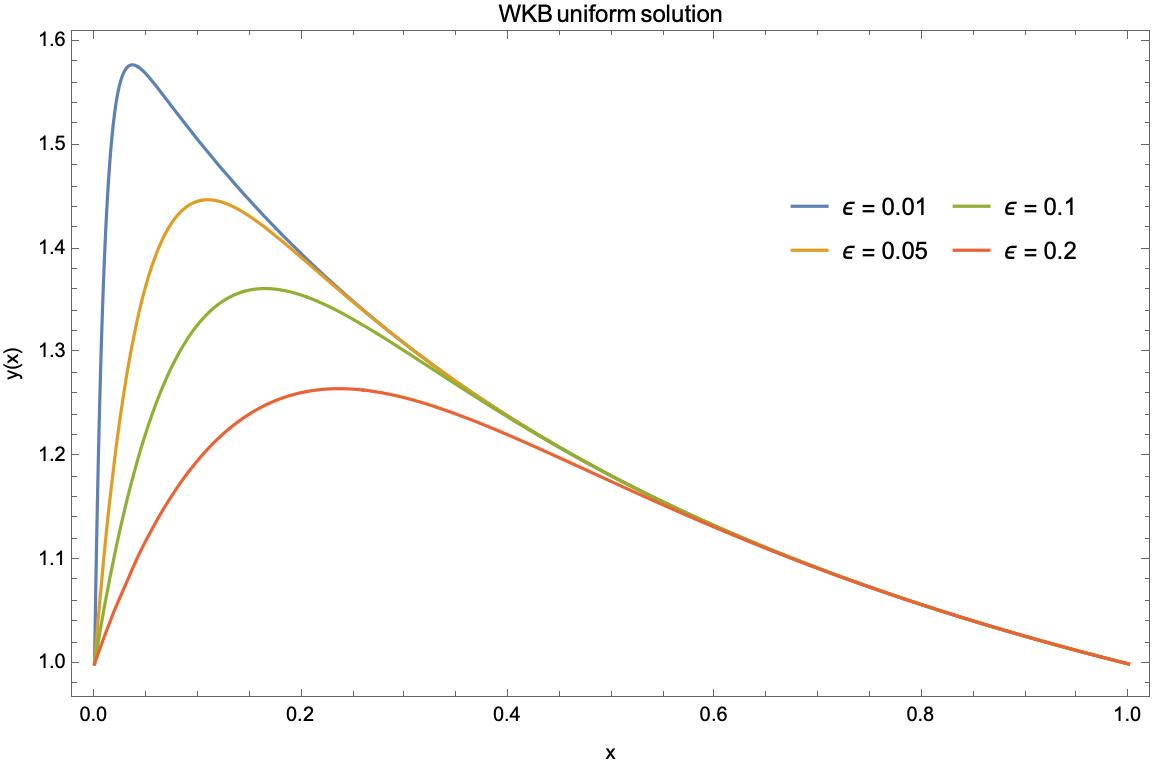
\includegraphics[width=14cm]{568_HW6_Plot.jpg}
            \caption{Leading order uniform solution for various values of $\epsilon$.}
        \end{figure}


    \end{enumerate}
\end{enumerate}

\end{document}